\section{Evaluation}
In this section, we will describe the experiences we had using the framework for three seperate applications; initial experiments using the crazyflie nano copter, a Wizard of Oz approach in which the frameworks correctness was verified, as well as a practical example using the more suitable AR Drone. Next, we present the results of a survey posted on various drone-related internet forums in order to gauge interest in the framework. Finally, we move on to evaluating the various properties of the architecture and the degree to which the framework does as envisioned.

\subsection{Practical Usage}
\subsubsection{Intial Experiments - The Crazyflie}
In the initial stages of this project, we experimented with developing drivers for the Crazyflie nano quadcopter, using the Microsoft Kinect for locationing. These efforts provided us with valuable knowledge on the current state of the art in regards to drone capabilities. Specifically, while the Crazyflie in and of itself was a suitable drone for freestyle flying, its rather limited control mechanisms and lack of hovering function severely impeded its use for the DroneCharge framework. It was very difficult if not impossible to make it land close enough to a charger for any real use, and task execution was unsafe at best. On a more positive note, it also gave us confidence that our driver-oriented architecture was correct, as the drivers were relatively straightforward to implement --- We just could not trust the drone to do as we commanded it. It also helped us define the granularity of the interface between the framework and the drone by giving us some experience with operating drones programatically, and some changes were made to the drivers in regards to the abstraction-level of drone control.

\subsubsection{Simulated approach - Wizard of Oz}
While our initial experiments gave us some more ideas on how to define the drone drivers, it did not allow us to physically test the framework. Instead, we focused on developing the framework by relying more on simulation and visualization for validation. We created visualization tools to illustrate the task tree as a coloured graph, and created a usage scenario in which a Microsoft Kinect tracked a drone. Rather than the drone moving itself, a Wizard of Oz approach was used in which a human actor purposefully moved the drone in the pattern indicated by the framework in order to perform the task. This was done using the video-feed from the Kinect and adding overlays with markings for the drone and its target position. For a video demonstration of the wizard of oz, we put a video on youtube which can be found in the footnotes \footnote{DroneCharge: https://www.youtube.com/watch?v=32yjwRk\_SrM}.

\begin{figure}[h]
\centering
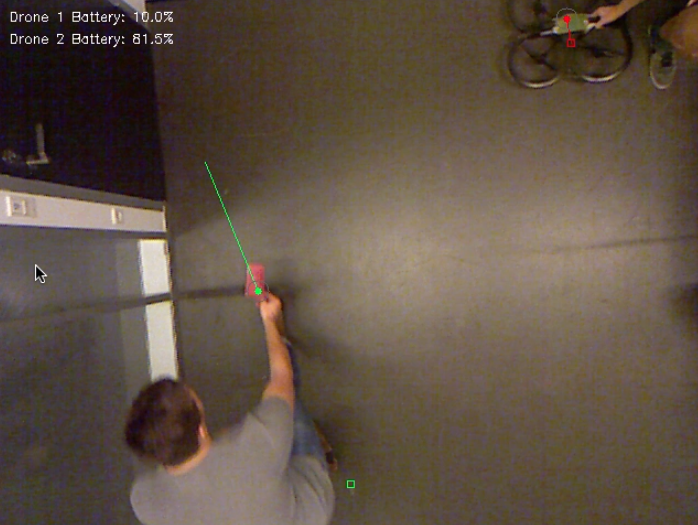
\includegraphics[width=\columnwidth]{images/wizardofoz.png}
\caption{Framework veritication using the Wizard of Oz approach for drone movement.}
\label{fig:wizardofoz}
\end{figure}

This approach allowed us to verify that the framework would act as intended provided that the drivers being used were implement as per specification.  While it was not as definitive proof as a real-life application, it provided us with enough verification to move on to a real drone.

\subsubsection{Practical Application - ARDrone}
Once the framework was in a relatively stable state, we went on to evaluate the framework by using it with an AR Drone. We kept the Kinect for tracking, and implemented the driver for the AR Drone. This was really straightforward, since we already had a driver for the Crazyflie. Where the Crazyflie was too unstable to reliably move around, the AR Drone had none of these problems. since the AR Drones API was essentially just a drop-in replacement, we only needed to import the AR Drone library\footnote{ARDrone: https://github.com/venthur/python-ardrone} and adapt the Crazyflie driver with a couple of lines of code.

The bulk of driver implementation was the translation between the locationing system into the Frameworks coordinates and vice versa. Because we had already written all of this for Crazyflie, swapping it for AR Drone was done in just a couple of hours with all the testing included. Apart from the method and class names that had to be changed, the only difference was in how the tilt angle is normalized before being passed on to the driver, which was just a trivial mathematical operation. The AR Drones firmware has proven to be much more stable than the Crazyflies. The drone was able to hold its position when asked, and responded to our commands well, which has resulted in a working prototype very quickly. Figure \ref{fig:ardrone} depicts an image of the drone being controlled by the framework. A video of the working prototype following a series of movement tasks can be found in the footnotes\footnote{DroneCharge: https://www.youtube.com/watch?v=Ei9mQTNHUgA}.

\begin{figure}[h]
\centering
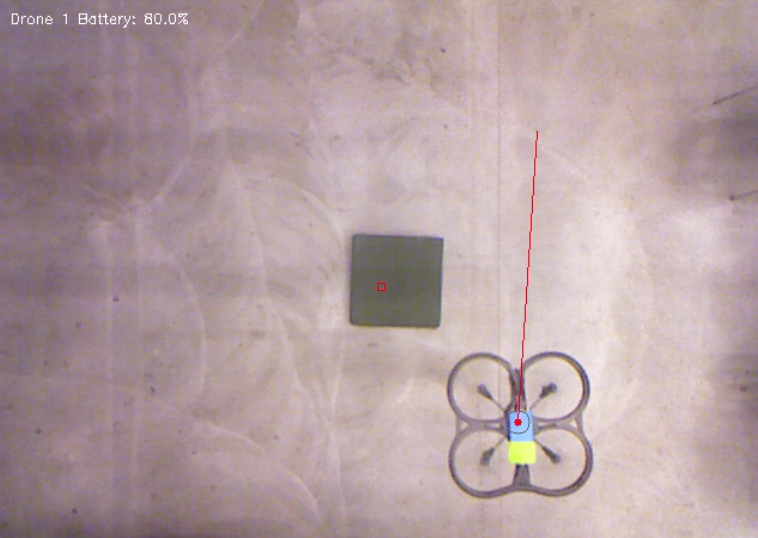
\includegraphics[width=\columnwidth]{images/drone.png}
\caption{AR Drone controlled by the framework}
\label{fig:ardrone}
\end{figure}

All in all, the driver was simple to implement, although we admittedly did have prior knowledge of the assumptions made for the drivers which simplified the process. However, the amount of code written to create the driver was almost neglible which speaks to the power of the approach. The code that we did have to write we would have written in any case if we were to do programmatic drone control.

\subsection{Developer survey}
To gauge whether this would be useful for real-world developers, we posted a survey along with a description of the system on several of the largest drone-development internet forums. Although only a limited amount of developers replied, five in total, we felt comfortable that the level of interest was adequate. 

When asked if the proposed framwork seemed useful, three developers replied that they either agreed or strongly agreed, one replied neutrally and one developer disagreed. When asked whether they had ever faced implementation issues that this framework would solve, three developers were neutral while one developer agreed and another strongly agreed. Finally, when asked if they would be interested in using such a framework, three developers agreed, one developer strongly agreed and only a single developer disagreed.

One developer also noted that our suggested way of positining the drone was inadequate, as drift would influence its absolute position. This caused us to reconsider our positioning and movement methods.

All in all, we believe it is safe to say that the interest in automatic charging of drones is present, although  responses may have been skewed by the possibility that only interested developers replied to the survey.

\subsection{Finding the Right Level of Abstraction}
In the beginning of the project, we wanted to also simplify drone-control implementation by only requiring the developer to implement atomic functions such as a command to move forward, fly up or down, or left or right. We would then supply high-level commands such as move to specific coordinates free of charge. However, we soon realized that drone control varies based on the type of drone, and that it was best to leave the specifics of controlling the drone to the implementer. While this left more responsibility to the implementer, which is arguably a negative property of a framework, it added a neccessary degree of flexibility. If we were to develop high-level commands, it would likely lead to less optimized flying routines and glitchy movement. Letting each individual developer do this allowed for very optimized flying for each individual type of drone. We also argue, that any drone implementer would need to implement drone controls to programatically utilize drones in either case, so the only thing our framework would then require, was that the control-code was written in a different location.

\subsection{Assumptions and Ease of Use}
As mentioned, we make several assumptions about both the driver implementation and the drones that are capable of using this framework. As a result, the ease of use, which should be a prime target for any framework, suffers. For example, knowing that individual tasks must not exceed the low battery level in terms of power usage is of paramount importance, but is not upheld in any way in the framework itself. An implementer would need to read documentation in order to know how to implement a task properly. Conclusively, the use of assumptions diminishes the level of intuitiveness of the framework.

\subsection{Flexibility}
The resulting framework is highly flexible. Theoretically, any type of copter-drone could be used in the framework. Even if the movement precision was very low, tasks that do not require very high movement precision could still be performed by expanding what constitutes a movement task as completed. For instance, by implementing a \textit{RoughMovementTask} which would be considered complete if the drone came within a certain range of the target. However, as the main purpose of the framework is to allow for recharging of drones, practicality demands that the drone be capable of landing within a relatively small area if automated charging was ever to occur.

\subsection{Recovery Options}
Currently, there are no fallback procedures if a drone enters an emergency state. This means, that if a drone was to somehow become unresponsive, e.g. by crashing into an obstacle, recovery is left solely to the developer. The main issue here stems from the fact that if we were to do recovery operations on the drone, that would mean that the drone was responsive, in which case the framework might as well continue with task execution.

On the other hand, if a drone were to be caught in a task, say for instance because a movement task attempted to fly the drone through a wall, there are no built-in contingencies to ensure that the task is ever completed. However, this could be handled in the drone driver by detecting abnormal behaviour and altering the route to the target.

\subsection{Collision detection and Environment mapping}
Currently, there is no notion of environment mapping. This means that for the framework to function, the area of operations must be a clear area with no  objects in the way. This is naturally not a pratical solution for real world tasks, but was decided for the purpose of simplicity. That there be no objects in the zone includes other drones, which causes problems when having several drones performing tasks or swapping with each other at the same time. This is, however, mainly a smaller issue as collision detection is something that is accounted for but was left as an additional module should time permit.

\subsection{Level of fulfillment}
We argue, that the framework set forth in this report fulfills the presented goals; it allows drone implementers to add automatic recharging and swarm behaviour to their drone-functionality with an acceptable level of additional code. While it does require the developer to adapt to our system of task execution rather than plug into their existing task execution methods, we argue that it is a small price to pay for the benefits gained by using DroneCharge.